%%% Local Variables: 
%%% mode: latex
%%% TeX-master: "../thesis"
%%% End: 

\section{Introduction}
\label{sec: moseg_introduction}
Progress in Dense Volumetric Fusion has been accelerated in recent years with
the availability of comsumer grade RGBD sensors such as the Microsoft Kinect and
the Asus Xtion coupled with the increasingly parallel nature of GPU hardware.
Systems such as the seminal KinectFusion \cite{Newcombe2011} allow one to build
high quality, globally consistent scene models trivially. Applications of such
reconstruction pipelines however are limited due to the inability of such
systems to handle scenes in which there are dynamics; such systems are unable
to yield reliable reconstructions when there is motion in the sensors field
of view independent of the sensors own motion. Such a scenario introduces
additional error to the Pose Estimation component in the pipeline and as such
causes model corruption.

In this chapter an approach to solving the problem of performing robust
Dense Volumetric Reconstruction in dynamic scenes is presented. Central to the
pipeline is the introduction of a dual scene representation based on the use
of an implicit TSDF \cite{Curless1996}. The use of a dual TSDF approach allows
for the segmentation of moving components in the scene from static components,
e.g. segmenting a person getting up from a chair from the chair itself. One of
the two scene representations is the ``static'' scene and the other the
``dynamic'' scene. Such separation prevents corruption in the static scene,
the reconstruction output of the system.

Without the segmentation of dynamic scene components, when tracking against the
current reconstruction the integrated dynamic components may cause artifacts
that prevent the finding of ICP correspondences which often causes camera
tracking to drift, or completely fail. By tracking against only the stable
scene components, this inteference in the ICP pose estimation process can be
mitigated.

Once a part of the dynamic model has been stable for a sufficient period, it's
volumetric data is integrated in to the static model and it is used for the
tracking phase of the pipeline. The use of Volumetric structures in this work
is motivated by previous works on Voxel Block Hashing \cite{NieBner2013},
providing efficient, real time lookup operations. The presented approach
exploits the abstraction that Voxel Blocks provide; a block of voxels is
interpreted as a region of space that can be either static or dynamic.
Voxel Block Stability is determined by a confidence measure over the Voxel
Blocks in the Dynamic Scene, such that Isosurface information is not transferred
to the Static Model(used for Camera Tracking) until there is sufficient
confidence in it's stability.
From a survey of the literature, it appears that this approach is the first to
utilise such a dual representation for the motion segmentation problem.

The remainder of this chapter is structured as follows.
Section \ref{sec:moseg_related_work} presents an assessment of related and
relevant literature. Section \ref{sec:moseg_static_fusion} introduces
preliminaries pertaining to the static Fusion pipeline followed by Section
\ref{sec:moseg_dynamic_fusion} describing the dynamic Fusion component of the
pipeline. Qualitative and Quantitative results are presented in Sections
\ref{sec:moseg_qualitative} and \ref{sec:moseg_quantitative}, respectively.
Finally, an application to interactive object recognition is given in Section
\ref{sec:moseg_semantic}.

\section{Related Work}
\label{sec:moseg_related_work}

\section{Static Volumetric Fusion}
\label{sec:moseg_static_fusion}
The Volumetric Fusion approach taken in this work draws on previous Volumetric
integration techniques \cite{Curless1996, Newcombe2011, NieBner2013,
  Prisacariu2014}
and shall be introduced in this section as preliminary material and shall be
referred to in later chapters. Following this approach, at each frame the camera
is tracked against the current scene, after which new data is fused into the
scene model which is then rendered using Raycasting to prepare for tracking in
the next frame.

The static Fusion pipeline consists of the following three consecutive steps:
\begin{itemize}
  \item Camera Tracking.
  \item Model Integration.
  \item Rendering.
\end{itemize}

The approach in this work utilises the TSDF Volumetric data structure which
encodes for each voxel in the structure, a signed value and a weight.
In the case of 3D environment modelling, the values pertain to distances from
surfaces, within some truncation region.

Given a vertex map generated from the back projection of the points in a depth
image, the vertices pertain to the zero crossing point with Voxels either side
representing distances to the zero crossing point; positive in front of the
surface, negative behind. Surface points are known as the Zero Level Set.
% TO-DO: make diagram.
For a given TSDF $\mathbf{\Phi}$, the Zero Level Set is defined as follows
\begin{equation}
  \label{eqn:zero_level_definition}
  \mathcal{S} = \{v \given \mathbf{\Phi}(v) = 0\}, 
  \mkern2mu \forall \mkern2mu v \in \mathbf{\Phi}
\end{equation}
where $v$ denotes a TSDF Voxel.

To facilitate real time fusion, the InfiniTAM framework employs a Voxel Block
Hashing mechanism for fast access to scene Voxels \cite{NieBner2013}. Within
this context, Voxel Blocks are collections of $N \times N \times N$ TSDF Voxels,
stored in a Hash Table for fast access. As such, each Hash Table entry
corresponds to a portion of a global Voxel Block Array, pertaining to a region
in the scene. This division of the scene into Voxel Blocks is used for the later
process of determining and labelling dynamic regions in the scene.

\subsection{Camera Tracking}
\label{subsec:moseg_static_camera_tracking}
As in previous works \cite{Newcombe2011, Prisacariu2014}, the gradient
optimisation based ICP algorithm is utilised to register consecutive images
to derive the camera pose at time $t$ with respect to time $t-1$, that is to
optimise for the Rigid Body Transform $\mathbf{T} \in \mathbb{SE}(3)$ of the
camera between the two frames using the Levenberg-Marquardt Nonlinear Least
Squares method \cite{NumericalRecipes}. The rendering stage of the pipeline
is used to generate the image from the TSDF  at time $t-1$ to which a new frame
at time $t$ is registered.

The target Transformation $\mathbf{T} \in \mathbb{SE}(3)$ is a member of the
Special Euclidean Group
\begin{equation}
  \label{eqn:se3_definition}
  \mathbb{SE}(3) = \{\mathbf{R}, \mathbf{t} \given \mathbf{R} \in
  \mathbb{SO}(3), \mathbf{t} \in \mathbb{R}^{3}\}
\end{equation}
and has the following form
\begin{equation}
  \label{eqn:trans_mat_definition}
  \mathbf{T} =
  \begin{bmatrix}
    \mathbf{R} & \mathbf{t} \\
    \mathbf{0} & 1
  \end{bmatrix}
\end{equation}
where $\mathbb{SO}(3)$ is the Special Orthogonal Group of Skew Symmetric
Rotation Matrices.

\subsubsection{Attitude Representation}
\label{subsub:moseg_static_camera_attitude}
The Rotation Matrix component of the Transformation $\mathbf{T}$ is
Generated by a Rodriguez Paramaterization\cite{Shuster1993}, whereby the
$\mathbb{SO}(3)$ Rotation Matrix $\mathbf{R}$ is generated by three rotational
parameters, $\alpha$, $\beta$ and $\gamma$. Each parameter represents a rotation
around one of three Principal Axes.

The formulation of the Rodriguez Paramaterization is given by the following 
\cite{Shuster1993}, with the parameter Vector
$\mathbf{p} = [\alpha, \beta, \gamma]^{T}$
\begin{equation}
  \label{eqn:rodriguez_matrix_eq}
  \mathbf{R}(\mathbf{p}) =
  \frac{1}{\norm{\mathbf{p}}^{2}}
  \bigg[
  (1 - \norm{\mathbf{p}}^{2})\mathbf{I} +
  2 \mathbf{pp}^{T} + \omega(\mathbf{p})
  \bigg]
\end{equation}
where for an arbitrary Vector $\mathbf{v}$, $\omega(\mathbf{v})$ is defined as
the Cross Product Matrix operator and is defined as follows
\begin{equation}
  \label{eqn:cross_prod_mat}
  \omega(\mathbf{v}) =
  \begin{bmatrix}
    0 & v_{3} & -v_{2} \\
    -v_{3} & 0 & v_{1} \\
    v_{2} & -v_{1} & 0
  \end{bmatrix}
\end{equation}

Evaluating Equation \ref{eqn:rodriguez_matrix_eq} leads to the following form
of the Rotation Matrix $\mathbf{R}$
\begin{equation}
  \label{eqn:rodriguez_matrix}
  \mathbf{R} = \frac{1}{\norm{\mathbf{p}}^{2} + 1}
  \begin{bmatrix}
    % Row 1.
    \alpha^{2} - \beta^{2} - \gamma^{2} + 1 &
    2 \alpha \beta + \gamma &
    2 \alpha \gamma - \beta \\
    % Row 2.
    2 \alpha \beta - \gamma &
    -(\alpha^{2} - \beta^{2} + \gamma^{2} - 1) &
    \alpha + 2 \beta \gamma \\
    % Row 3.
    2 \alpha \gamma + \beta &
    -(\alpha - 2 \beta \gamma) &
    -(\alpha^{2} + \beta^{2} - \gamma^{2} - 1)
  \end{bmatrix}
\end{equation}

The Translational component $\mathbf{t}$ of the Transformation $\mathbf{T}$ is
given by the following Vector, with each component representing a translation
along it's respective axis.
\begin{equation}
  \label{eqn:trans_vector}
  \mathbf{t} =
  \begin{bmatrix}
    t_{x} \\
    t_{y} \\
    t_{z}
  \end{bmatrix}
\end{equation}

\subsubsection{Pose Recovery Formulation}
\label{subsub:moseg_static_camera_poserec}
The recovery of the camera pose change between frames $t$ and $t-1$ may be
formulated as the following Energy Minimisation problem
\begin{equation}
  \label{eqn:pose_estimation_kf}
  E(\mathbf{R}, \mathbf{t}, \mathbf{\Omega}, \mathbf{\Phi}) =
  \argmin_{\mathbf{R}, \mathbf{t}} \sum_{p \in \mathbf{\Omega}}
  \norm{\left[
    \mathbf{Rx} + \mathbf{t} - \mathcal{V}(\bar{\mathbf{x}})
  \right]^{T}
  \mathcal{N}(\bar{\mathbf{x}})}
\end{equation}
where $\mathbf{R}$ and $\mathbf{t}$ are the aforementioned Rotation Matrix and
Translation Vector of the transformation $\mathbf{T}$. $\mathbf{x}$ is the 3D
point extracted from the depth image $\mathbf{\Omega}$ and the point
$\bar{\mathbf{x}}$ is the 3D point in the TSDF Volume $\mathbf{\Phi}$ found by
Raycasting from $\mathbf{\Omega}$ under the Transformation $\mathbf{T}$.
Finally, $\mathcal{N}$ is a Normal map of $\mathbf{\Phi}$ and is defined as
follows
\begin{equation}
  \label{eqn:normal_map_definition}
  \mathcal{N} = \frac{\nabla \mathbf{\Phi}}{\norm{\nabla \mathbf{\Phi}}}
\end{equation}
where $\nabla \mathbf{\Phi}$ is approximated with Central Finite Differencing.

For the Gradient update phase of the ICP algorithm, the Partial Derivatives
$\frac{\partial E}{\partial \mathbf{R}_{\{\alpha, \beta, \gamma\}}}$ may be
derived as follows in Equation \ref{eqn:icp_update_derivation}.
As a first step, the following definition is made
\begin{equation}
  \label{eqn:icp_deriv_sub}
  \phi(\mathbf{R}, \mathbf{t}, \mathbf{x}, \bar{\mathbf{x}}) =
  \left[
    \mathbf{Rx} + \mathbf{t} - \mathcal{V}(\bar{\mathbf{x}})
  \right]^{T}
  \mathcal{N}(\bar{\mathbf{x}})
\end{equation}
With this substitution in place, the derivation proceeds as follows
\begin{equation}
  \label{eqn:icp_update_derivation_rot}
  \begin{split}
    % Line 1.
    \frac{\partial E}{\partial \mathbf{R}_{\{\alpha, \beta, \gamma\}}} & =
    \frac{\partial}{\partial \mathbf{R}_{\{\alpha, \beta, \gamma\}}}
    \sum_{p \in \mathbf{\Omega}}
    \norm{\phi(.)}\\
    % Line 2.
    & = \sum_{p \in \mathbf{\Omega}}
    \frac{\partial}{\partial \mathbf{R}_{\{\alpha, \beta, \gamma\}}}
    \norm{\phi(.)}\\
    % Line 3.
    & = \sum_{p \in \mathbf{\Omega}}
    \frac{\partial}{\partial \phi(.)} \norm{\phi(.)}
    \frac{\partial \phi(.)}{\partial \mathbf{R}_{\{\alpha, \beta, \gamma\}}}\\
    % Line 4.
    & = \sum_{p \in \mathbf{\Omega}}
    \frac{1}{2}\frac{2 \phi(.)}{\sqrt{\phi(.)^{T}\phi(.)}}
    \frac{\partial \phi(.)}{\partial \mathbf{R}_{\{\alpha, \beta, \gamma\}}}\\
    % Line 5.
    & = \sum_{p \in \mathbf{\Omega}}
    \frac{\phi(.)}{\norm{\phi(.)}}
    \frac{\partial \phi(.)}{\partial \mathbf{R}_{\{\alpha, \beta, \gamma\}}}\\
    % Line 6
    & = \sum_{p \in \mathbf{\Omega}}
    \frac{\phi(.)}{\norm{\phi(.)}}
    \Bigg[ \frac{\partial}{\partial \mathbf{R_{\{\alpha, \beta, \gamma\}}}}
    \bigg[ \mathbf{Rx} + \mathbf{t} - \mathcal{V}(\bar{\mathbf{x}}) \bigg]^{T}
    \mathcal{N}(\bar{\mathbf{x}}) + 
    \bigg[ \mathbf{Rx} + \mathbf{t} - \mathcal{V}(\bar{\mathbf{x}}) \bigg]^{T}
    \frac{\partial}{\partial \mathbf{R}_{\{\alpha, \beta, \gamma\}}}
    \mathcal{N}(\bar{\mathbf{x}})\Bigg]\\
    % Line 6
    & = \sum_{p \in \mathbf{\Omega}}
    \frac{\phi(.)}{\norm{\phi(.)}}
    \bigg[ \frac{\partial \mathbf{R}}{\partial \{\alpha, \beta, \gamma\}}
    \mathbf{x}\bigg]^{T}
    \mathcal{N}(\bar{\mathbf{x}})
  \end{split}
\end{equation}
The full Partial Derivatives $\frac{\partial \mathbf{R}}{\partial \alpha}$,
$\frac{\partial \mathbf{R}}{\partial \beta}$ and
$\frac{\partial \mathbf{R}}{\partial \gamma}$ may be found Equations
\ref{eqn:rodrigues_full_alpha_deriv}, \ref{eqn:rodrigues_full_beta_deriv}
and \ref{eqn:rodrigues_full_gamma_deriv} of Appendix 
\ref{appendix:mathematical}.

The Partial Derivatives
$\frac{\partial \mathbf{R}}{\partial \{\alpha, \beta, \gamma\}}$ may be
multiplied with $\mathbf{x}$ and combined in to the following Rotation Jacobian
\begin{equation}
  \label{eqn:rot_jac}
  \begin{split}
    \mathbf{J}_{R} & = \left. \bigg[
      \frac{\partial \mathbf{R}}{\partial \{\alpha, \beta, \gamma\}} \mathbf{x}
      \bigg]^{T} \right\vert_{\alpha,\beta,\gamma = 0} \\
    & =
    \begin{bmatrix}
      0 & -z & y \\
      z & 0 & -x \\
      -y & x & 0
    \end{bmatrix}
  \end{split}
\end{equation}

Note that the derivation for the Partial Derivatives
$\frac{\partial E}{\partial \mathbf{t}_{\{x, y, z\}}}$ is analogous with that of
Equation \ref{eqn:icp_update_derivation_rot}, with the result given as follows
\begin{equation}
  \label{eqn:icp_update_derivation_trans}
  \frac{\partial E}{\partial \mathbf{t}_{\{x, y, z\}}} =
  \sum_{p \in \mathbf{\Omega}}
  \frac{\phi(.)}{\norm{\phi(.)}}
  \bigg[ \frac{\partial \mathbf{t}}{\partial \{x, y, z\}}\bigg]^{T}
  \mathcal{N}(\bar{\mathbf{x}})
\end{equation}

The Translation Partial Derivatives
$\frac{\partial \mathbf{t}}{\partial \{x, y, z\}}$ may also be combined in to
the following Translation Jacobian
\begin{equation}
  \label{eqn:trans_jac}
  \mathbf{J}_{t} =
  \begin{bmatrix}
    1 & 0 & 0 \\
    0 & 1 & 0 \\
    0 & 0 & 1
  \end{bmatrix}
\end{equation}

The overall combined Jacobian for the Energy function defined in Equation
\ref{eqn:pose_estimation_kf} as follows
\begin{equation}
  \label{eqn:pose_jacobian}
  \mathbf{J} =
  \frac{\phi(.)}{\norm{\phi(.)}}
  \begin{bmatrix}
    \mathbf{J}_{R} & \mathbf{J}_{t}
  \end{bmatrix}^{T}
  \mathcal{N}(\bar{\mathbf{x}})
\end{equation}

\subsubsection{Pose Recovery Optimisation}
\label{subsub:moseg_static_camera_poserec_opt}
With the gradient derivations in place, this section will now detail the
Pose Recovery procedure. As highlighted, the optimisation routine used is the
Levenberg-Marquardt\cite{NumericalRecipes} algorithm for solving Nonlinear Least
Squares problems. The Gradient update equation for the Levenberg-Marquardt
algorithm is given as follows
\begin{equation}
  \label{eqn:lm_update}
  \theta_{t+1} = \theta_{t} - (\mathbf{H} + \lambda \text{diag}(
  \mathbf{H}))^{-1}
  \mathbf{J}
\end{equation}
where $\theta_{t} = [\alpha, \beta, \gamma, t_{x}, t_{y}, t_{z}]^{T}$ is the
Parameter Vector of $\mathbf{T}$ at time $t$, $\mathbf{J}$ is the Jacobian
introduced in Equation \ref{eqn:pose_jacobian} and $\mathbf{H}$ is the Hessian,
approximated by $\mathbf{H} = \mathbf{J}^{T}\mathbf{J}$. The parameter $\lambda$
controls the influence of the Gradient on the update step and is adjusted
according to the change in error, as shall be evident in the Algorithm
that follows.

{
  \centering
  \singlespacing
  \begin{minipage}{.7\linewidth}
    \begin{algorithm}[H]
      \label{alg:icp}
      \caption{ICP with Levenberg-Marquardt}
      \begin{algorithmic}[1]
        \Procedure{ICP}{$\mathcal{D}_{l}, \mathcal{D}_{m}, \mathcal{V},
          \theta_{t-1}$}
        \State $\lambda \gets \lambda_{init}$
        \State $\theta_{tmp} \gets \theta_{t-1}$
        \State $\theta_{t} \gets \theta_{tmp}$
        \State $\epsilon_{old} \gets \inf$
        \State $\epsilon \gets \epsilon_{old}$
        \While{$\epsilon >= \tau$}
        \State $\epsilon \gets E(.)$
        \Comment{Evaluate Equation \ref{eqn:pose_estimation_kf}}
        \If{$\epsilon \leq \epsilon_{old}$}
        \State $\lambda \gets 10\lambda$
        \State $\theta_{t} \gets \theta_{tmp}$
        \Else
        \State $\lambda \gets \frac{\lambda}{10}$
        \State $\epsilon_{old} \gets \epsilon$
        \State $\theta_{tmp} \gets \theta_{t}$
        \EndIf
        \State $\mathbf{J} \gets \nabla E$
        \Comment{Evaluate Equation \ref{eqn:pose_jacobian}}
        \State $\mathbf{H} = \mathbf{J}^{T}\mathbf{J}$
        \State $\mathbf{C} = \text{chol}(\mathbf{H} +
        \lambda \text{diag}(\mathbf{H}))$
        \State $\delta = \text{backsub}(\mathbf{C}, \mathbf{J})$
        \State $\theta_{tmp} \gets \theta_{tmp} - \delta$
        \EndWhile\\
        \Return $\theta_{t}$
        \EndProcedure
      \end{algorithmic}
    \end{algorithm}
  \end{minipage}
  \par
}

\subsection{Volumetric Integration}
\label{subsec:moseg_static_integration}
The second phase in the Scene Reconstruction pipeline is Volumetric Integration.
That is, the integration of observed depth images in to a consistent, Implicit
Volumetric representation, in this case the existing TSDF model of the scene,
providing the basis for an updated rendering to be used in the ICP procedure
for Tracking at the next time step.

As previously outlined, the TSDF may be defined as a volume of distances to an
Isosurface, with the Isosurface itself being given by the Zero Level Set, as
defined in Equation \ref{eqn:zero_level_definition}. A graphical representation
is given in Figure \ref{fig:sdf_example}.
% Based on: http://www.texample.net/tikz/examples/contours-grids/
\begin{figure}[h]
  \label{fig:sdf_example}
  \centering
  TODO: Make figure.
  \caption{An example of a Two Dimensional Signed Distance Function.}
\end{figure}

As with KinectFusion \cite{Newcombe2011} the global (scene) location
$\mathbf{x}_{v}$ of each voxel $v \in \mathbf{\Phi}$ that is visible in the
current view frustum is transformed into the camera's coordinate frame via the
following Transformation(noting that $\mathbf{x}_{v}$ is in Homogeneous form)
\begin{equation}
\label{eqn:project_tsdf_to_image}
\mathbf{x}_{\Omega} = \mathbf{K}\mathbf{T}_i^{-1}\mathbf{x}_{v}
\end{equation}
where $\mathbf{K}$ is the Camera's Intrinsic Calibration Matrix, $\mathbf{T}$ is
the Transformation optimised for at time $t$, with the form given in Equation
\ref{eqn:trans_mat_definition} and $\mathbf{x}_{\Omega}$ is the resultant
projected coordinates.

The Integration of new data points into the TSDF Volume is achieved by computing 
running averages; each voxel contains a running average of its SDF value over
time.

Projecting to the depth image $\mathbf{\Omega}$ coordinates as in Equation
\ref{eqn:project_tsdf_to_image} to perform a depth lookup in $\mathbf{\Omega}$
and subtracting the $z$ component of $\mathbf{x}_{v}$ from the resulting value
yields the depth offset from the surface, as follows
\begin{equation}
  \label{eqn:integration_offset}
  \eta = \mathbf{x}_{\Omega} - \mathbf{x}_{v}^{z}
\end{equation}

If $\eta \geq -\mu$, that is that the depth of the point is not beyond the
truncation band behind the Isosurface(Zero Level Set), where $\mu$ is half the
width of the truncation band, then the TSDF depth measurement update proceeds as
follows for a Voxel $\mathbf{x}_{v} \in \mathbf{\Phi}$.
\begin{equation}
\label{eqn:sdf_update}
\mathbf{\Phi}(\mathbf{x}_{v})_{t} = \frac{1}{\phi(\mathbf{x}_{v})_{t-1} + 1}
\bigg[\phi(\mathbf{x}_{v})_{t-1}\mathbf{\mathbf{\Phi}}(\mathbf{x}_{v})_{t-1} +
\text{min} \bigg( 1, \frac{\eta}{\mu} \bigg)
\bigg]
\end{equation}
In addition, the weight $\phi(\mathbf{x}_{v})$ is updated as follows.
\begin{equation}
  \label{eqn:sdf_weight_update}
  \phi(\mathbf{x}_{v})_{t} = \phi(\mathbf{x}_{v})_{t-1} + 1
\end{equation}

\subsection{Rendering}
\label{subsec:moseg_static_rendering}
Following the Integration process outlined in Section
\ref{subsec:moseg_static_integration} is the rendering stage in which an image
of the scene image is generated to provide an updated view for the tracking
stage outlined in Section \ref{subsec:moseg_static_camera_tracking}, at the next
time step.

Rendering in the pipeline is achieved by Raycasting, the process of `casting` a
ray from the Camera Frame into the scene, to find intersections with the scene
Isosurface. 
% A complete treatment of the Raycasting procedure may be found in the computer
% graphics literature \cite{Parker:1998:IRT:288216.288266}.

\section{Volumetric Fusion with Dynamic Scenes}
\label{sec:moseg_dynamic_fusion}
To adapt the conventional approach described in Section
\ref{sec:moseg_static_fusion} to handle dynamic environments, a dual-volume
representation of the scene is introduced, consisting of a \emph{Static Model}
and a \emph{Dynamic Model} (both of which are TSDF's).

There are two additional stages in the dynamic pipeline to handle integration in
to the Static Model. The first updates stability values for all of the Voxel
Blocks in the current view frustum at each frame. The second Integrates blocks
whose stability values are above a certain threshold into the static model.
Camera Tracking is performed against the Static Model as soon as it contains
valid Isosurface data to track against, preventing moving objects in the scene
from contributing to tracking drift.

An overview of the Pipeline is given in Figure \ref{fig:moseg_pipeline}
\begin{figure}[h]
  \label{fig:moseg_pipeline}
  \centering
  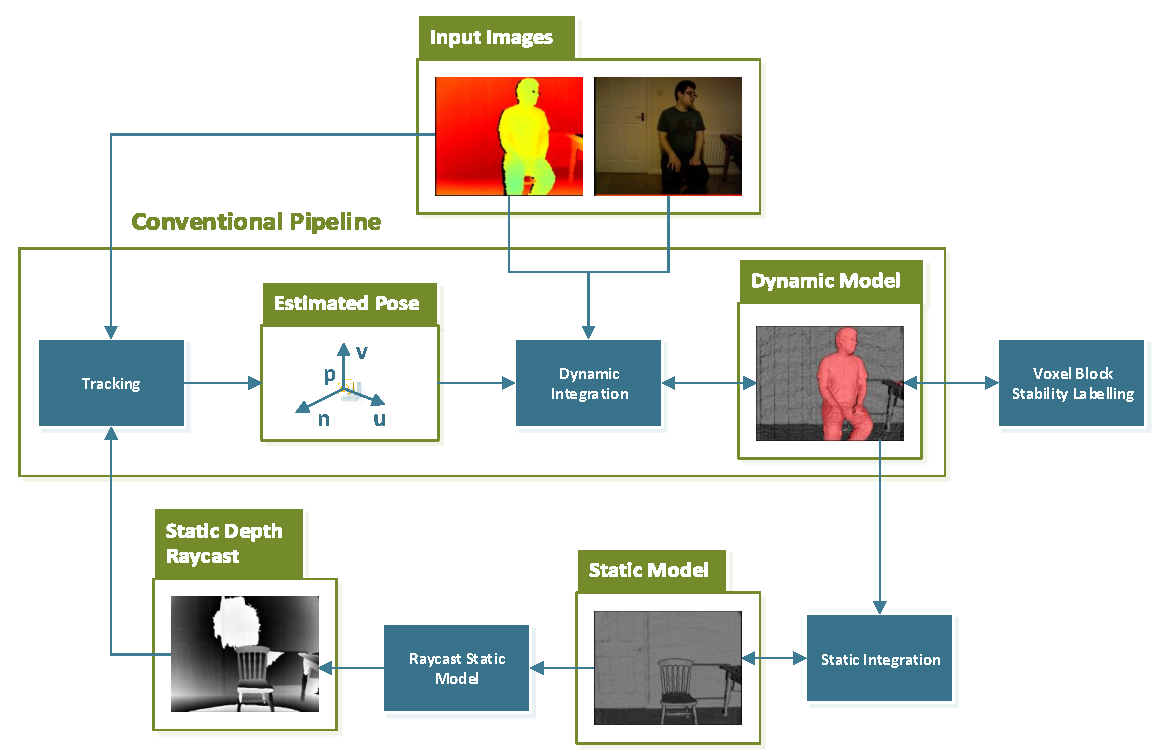
\includegraphics[width=\linewidth]{figures/moseg/pipeline.pdf}
  \caption{The Motion Segmentation pipeline. Note the additional Voxel Block
    Labelling stage with a feedback to the Model Integration stage.}
\end{figure}

\subsection{Stability Labelling}
\label{sub:moseg_stability_labelling}
The purpose of the stability labelling section of the pipeline is to distinguish
between Stable and Unstable Voxel Blocks in the Dynamic Model, resulting in
parts of the scene that are moving being excluded from the Static Model.

For each Voxel Block in the Dynamic Model, a \emph{Stability Value} is
maintained, representing the extent to which the instantaneous TSDF values for
the Voxels in a given Voxel Block(visible in the current View Frustrum under the
current Pose) have remained similar to the existing TSDF values for those voxels
over time.

The stability value for each voxel block in the scene is initialised to nought.
At each frame, the instantaneous TSDF values for the Voxels in each visible
Voxel Block are computed. For each Voxel Block, the Mean Absolute Difference
$\tau$, between the instantaneous and existing TSDF values is computed as
follows.
\begin{equation}
  \label{eqn:moseg_stability_value}
  \tau_{\mathcal{V}} = \Bigg[ \frac{1}{|\mathcal{V}|} \sum_{v \in \mathcal{V}}
  \bigg|\mathbf{\Phi}^{d}(v) - \text{min}\bigg(1, \frac{\eta}{\mu}\bigg)\bigg| \Bigg]
\end{equation}
The Stability Label $l_{\mathcal{V}} \in \{\text{stable}, \text{unstable}\}$ for
a given Voxel Block $\mathcal{V}$ is determined by thresholding on $\xi$
(empirically set to $0.3m$) as follows.
\begin{equation}
  \label{eqn:moseg_stability_labelling}
  l_{\mathcal{V}} =
  \begin{cases}
    \text{stable} & \textbf{if} \mkern4mu \tau \leq \xi \\
    \text{unstable} & \textbf{if} \mkern4mu \tau > \xi
  \end{cases}
\end{equation}
If the label $l_{\mathcal{V}}$ is ``stable'', the implication is that the Voxel
Block contains few disparities between the current scene and the stored model.
In this case, it's stability value is incremented. If however
$l_{\mathcal{V}}$ has the label ``unstable'', the implication is that the
contents of the Voxel Block are changing, so it's stability value is reset to
nought, as follows.
\begin{equation}
  \label{eqn:moseg_stability_update}
  \tau_{\mathcal{V}} =
  \begin{cases}
    \tau_{\mathcal{V}} + 1 & \textbf{if} \mkern4mu l_{\mathcal{V}} =
    \text{stable}\\
    0 & \textbf{if} \mkern4mu l_{\mathcal{V}} = \text{unstable}
  \end{cases}
\end{equation}

Voxel Blocks that are observed to be stable over a sufficiently long period of
time (empirically set to $40$ frames) will be Integrated into the Static Model,
as follows in Section \ref{sub:moseg_static_to_dynamic}.

\subsection{Integration into Static Model from Dynamic Model}
\label{sub:moseg_static_to_dynamic}
For a time step $t$, each Voxel Block in the Dynamic Model that has assigned to
it a stable label has the entirety its Voxel TSDF values Integrated in to the
static model. In a similar formulation to that of Equation \ref{eqn:sdf_update}
in Section \ref{subsec:moseg_static_integration}, the update comprises
Integration of new data in to a running average.

The weight update for a given Voxel $v$ in the Stable Model $\mathbf{\Phi}^{s}$
with respect to a Voxel(belonging to a Voxel Block labelled ``stable'') 
$\bar{v}$ in the Dynamic Model $\mathbf{\Phi}^{d}$ is given as follows.
\begin{equation}
  \label{eqn:moseg_weight_update}
  \phi^{s}_{t}(v) = \phi(v)^{s}_{t-1}(v) + \phi(\bar{v})^{d}_{t-1}(\bar{v})
\end{equation}
Similarly, the update for the TSDF values is as follows.
\begin{equation}
  \label{eqn:moseg_sdf_update}
  \mathbf{\Phi}^{s}_{t}(v) = \frac{1}{\phi^{s}_{t}(v)} \bigg[
  \phi^{s}_{t-1}(v) \mathbf{\Phi}^{s}_{t-1}(v) +
  \phi^{d}_{t-1}(\bar{v}) \mathbf{\Phi}^{d}_{t-1}(\bar{v})
  \bigg]
\end{equation}

\section{Qualitative Results}
\label{sec:moseg_qualitative}
Empirically, the proposed Motion Segmentation system is capable of retaining
globally consistent tracking within the Dense SLAM framework for a range of
scenarios that would prove to be problematic for other, static Dense SLAM
systems. The experiments performed demonstrate a robustness	to dynamics in
various scenes, both in terms of tracking and noise artefacts in the static
model. In addition, the system is robust to the addition and removal of scene
components and is robust to short term occlusions, such as a person walking in
front of the camera. An example of a person moving in to the the View Frustrum
and sitting on a Setee is given in Figure \ref{fig:moseg_qualitative_setee}.

\begin{figure}[h]
  \label{fig:moseg_qualitative_setee}
  \centering
  \begin{tabular}{ccc}
    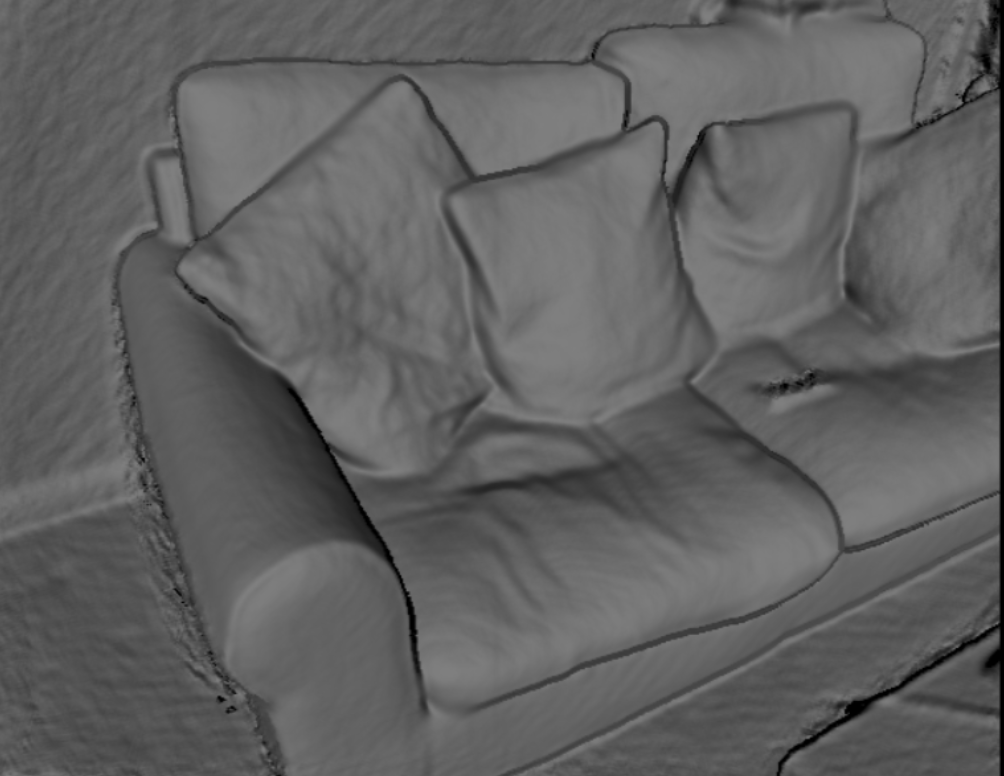
\includegraphics[height=.2\linewidth]{figures/moseg/original_sitting.png} &
    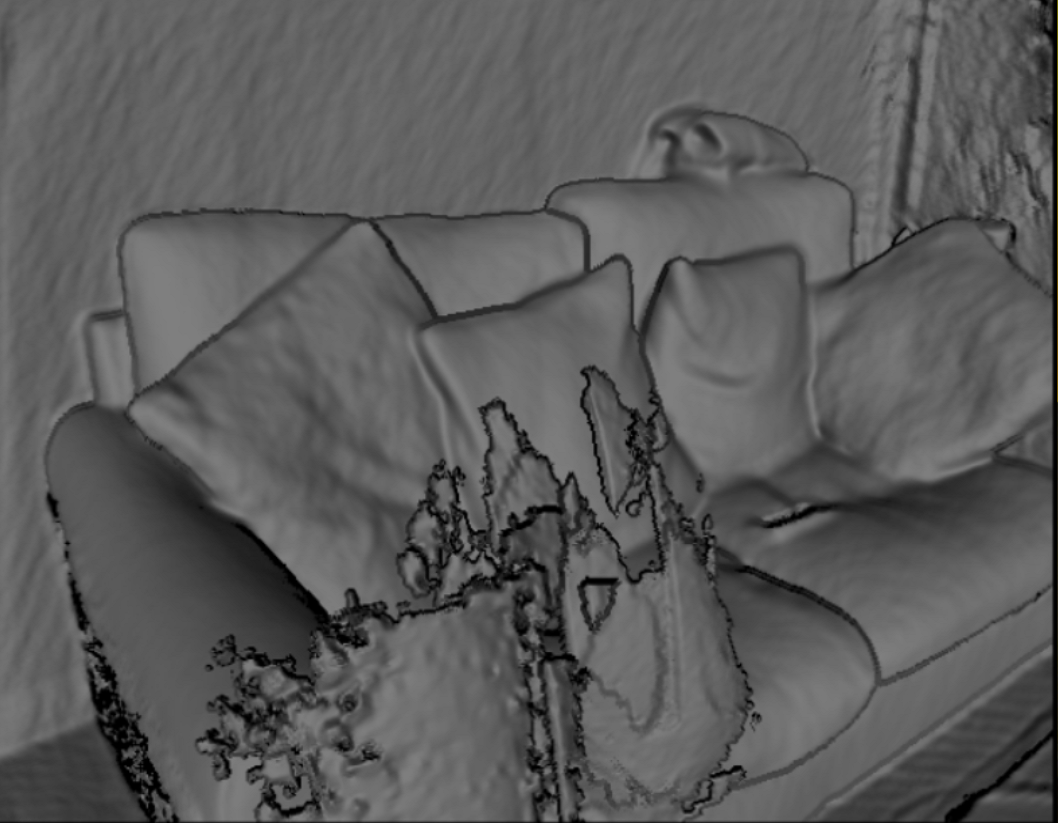
\includegraphics[height=.2\linewidth]{figures/moseg/infinitam_sitting.png} &
    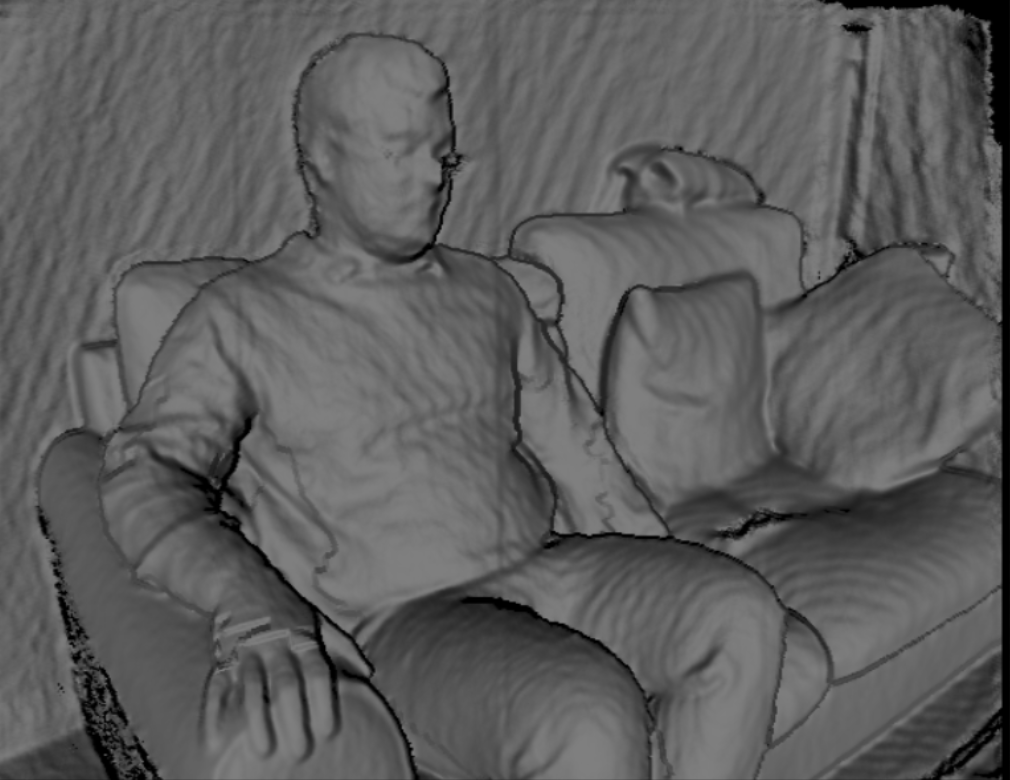
\includegraphics[height=.2\linewidth]{figures/moseg/moseg_sitting.png}\\
    (a) & (b) & (c)
  \end{tabular}
  \caption{A qualitative comparison between the proposed system and InfiniTAM
    \cite{Prisacariu2014}.
    (a) A static scene containing a Setee is reconstructed.
    (b) When a person enters the scene using standard InfiniTAM, the tracking
    fails, leading to a corrupted scene model.
    (c) Using the proposed system, tracking is maintained and the person is
    Integrated successfully into the scene.}
\end{figure}

In addition to the ability to reconstruct a moving object that becomes static in
the scene as shown in Figure \ref{fig:moseg_qualitative_setee}, the proposed
system is also capable of segmenting dynamic objects in a scene that are
undergoing nonrigid motion. Whilst these objects are segmented and labelled as
``dynamic'' they are not used for Camera Pose Estimation. An example of this
behaviour may be observed in Figure \ref{fig:moseg_qualitative_chair}.

\begin{figure}[h]
  \label{fig:moseg_qualitative_chair}
  \centering
  \begin{tabular}{cc}
    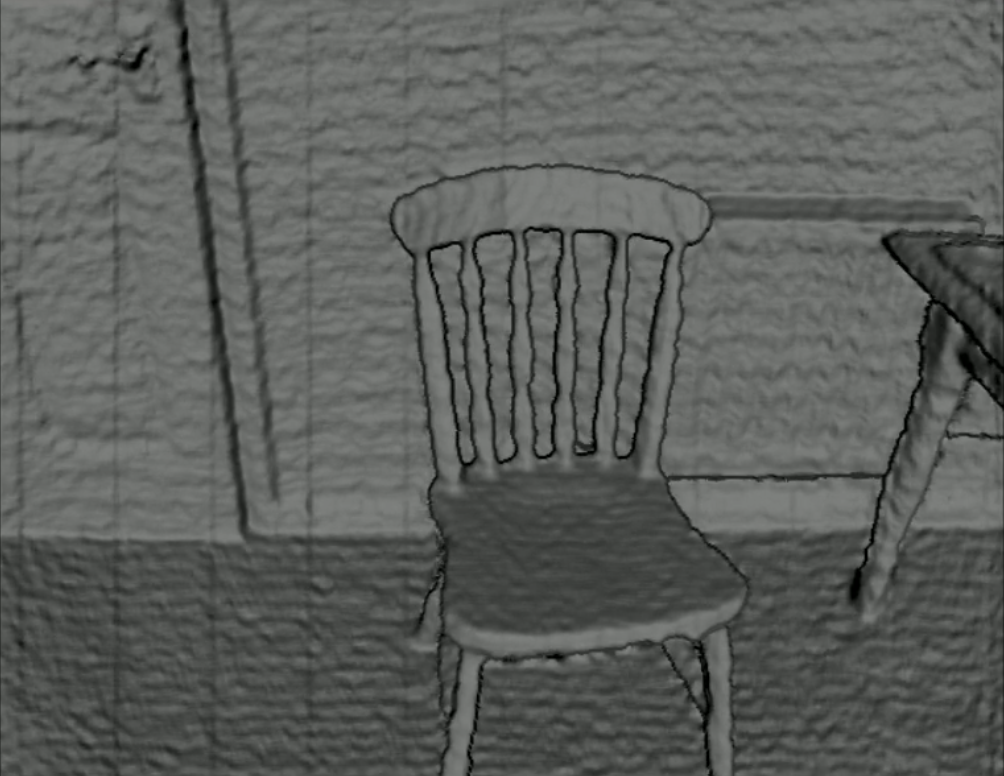
\includegraphics[height=.25\linewidth]{figures/moseg/chair0.png} &
    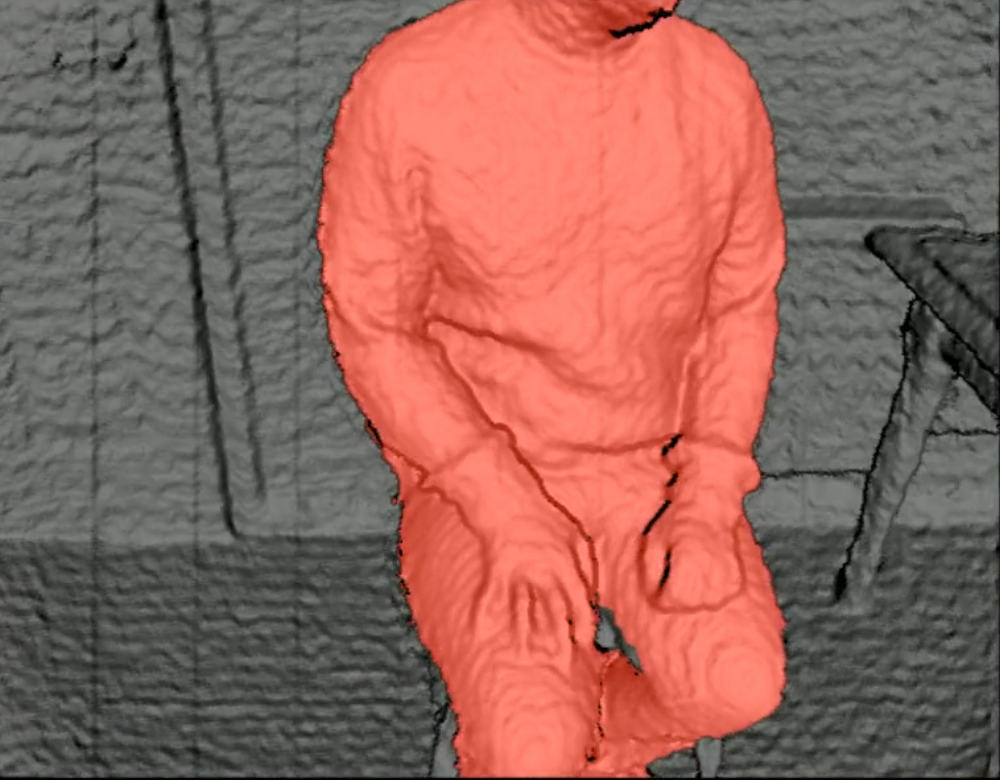
\includegraphics[height=.25\linewidth]{figures/moseg/chair1.png} \\
    (a) & (b) \\
    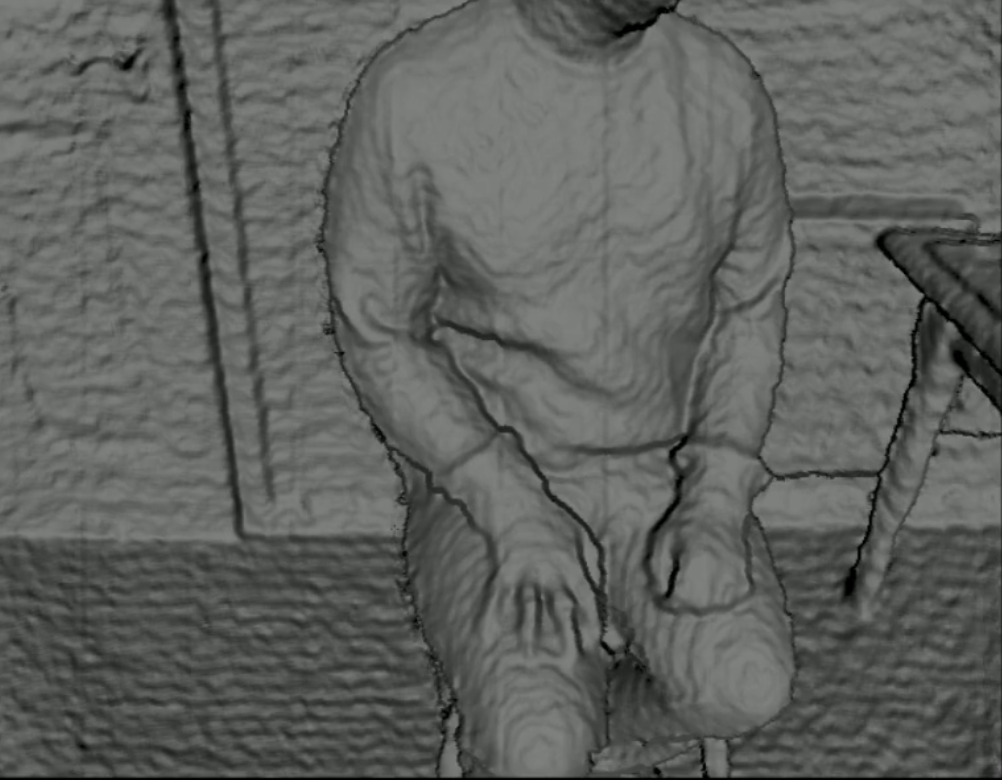
\includegraphics[height=.25\linewidth]{figures/moseg/chair2.png} &
    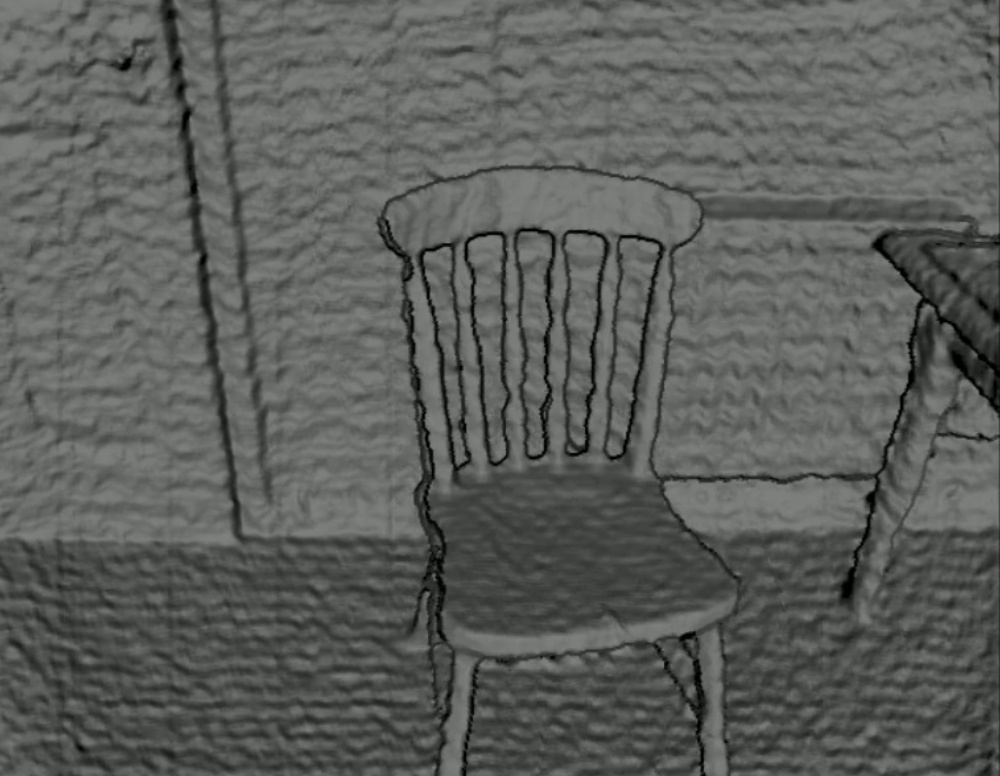
\includegraphics[height=.25\linewidth]{figures/moseg/chair3.png} \\
    (c) & (d)
  \end{tabular}
  \caption{A qualitative example of the proposed systems ability to segment
    dynamic scene components.
    (a) A static scene containing a Chair is reconstructed.
    (b) A person enters the scene, is marked as ``dynamic'' and sits down.
    (c) After gaining a sufficient confidence score, the person is labelled
    ``static'' and is integrated in to the Static Model.
    (d) The person gets up from the Chair and leaves the scene. The original
    reconstruction of the chair from (a) is in tact.}
\end{figure}

\section{Quantitative Results}
\label{sec:moseg_quantitative}
In this section, a quantitative evaluation of the system's efficacy in terms of
and Camera Tracking ability is provided.

For the quantitative analysis, the system has been evaluated on the Dynamic
Objects subset of the TUM RGBD dataset \cite{Sturm2012} with respect to
trajectory quality. The scenes provided in the dataset contain a range of
dynamic components ranging from arm movement to people walking around, occluding
parts of the scene. Comparison is drawn against the standard InfiniTAM framework
on which the proposed system is based, using standard, static InfiniTAM as a
baseline.

\begin{table}[h]
  \label{tbl:moseg_ate}
\begin{center}
  \begin{tabular}{l@{\hskip 1cm} c c}
    \emph{TUM Standard Sequence Name} & \emph{MoSeg} ATE & \emph{Baseline} ATE \\
    \midrule
    \textsf{fr2-desk-with-person} & \textbf{0.158 \std{0.091}} & 0.297 \std{0.193}\\
    \textsf{fr3-sitting-static} & 0.014 \std{0.008} & \textbf{0.012 \std{0.007}}\\
    \textsf{fr3-sitting-xyz} & 0.064 \std{0.031} & \textbf{0.053 \std{0.029}}\\
    \textsf{fr3-sitting-halfsphere} & 0.142 \std{0.063} & \textbf{0.115 \std{0.049}}\\
    \textsf{fr3-sitting-rpy} & \textbf{0.056 \std{0.033}} & 0.081 \std{0.051}\\
    \textsf{fr3-walking-static} & \textbf{0.294 \std{0.153}} & 0.999 \std{0.178}\\
    \textsf{fr3-walking-xyz} & \textbf{0.385 \std{0.271}} & 0.544 \std{0.343}\\
    \textsf{fr3-walking-halfsphere} & \textbf{0.539 \std{0.360}} & 0.762 \std{0.367}\\
    \textsf{fr3-walking-rpy} & \textbf{0.662 \std{0.335}} & 0.843 \std{0.365}\\
  \end{tabular}
\end{center}
\caption{The Bbsolute Trajectory Error (ATE) results (in metres, lower is better
  ) achieved by the proposed approach in comparison to the baseline InfiniTAM
  \cite{Prisacariu2014} framework on a variety of the standard sequences from
  the TUM RGBD dataset \cite{Sturm2012}. Results are in the format mean
  $\pm$ standard deviation. The better result (by mean) on each sequence is
  highlighted in bold.}
\end{table}

Given in Table \ref{tbl:moseg_ate} is the Absolute Trajectory Error measures
for each of the TUM Dynamic Scenes. The Absolute Trajectory Error utilises the
method of Horn \cite{Horn1987} to solve for the error incurred by mapping the
trajectory of the proposed system on to the ground truth trajectory of the TUM
sequence, for a given TUM Dynamic Objects sequence.

The results of Table \ref{tbl:moseg_ate} are visualised in Figure
\ref{fig:moseg_ate}.

\begin{figure}[h]
  \label{fig:moseg_ate}
  \centering
  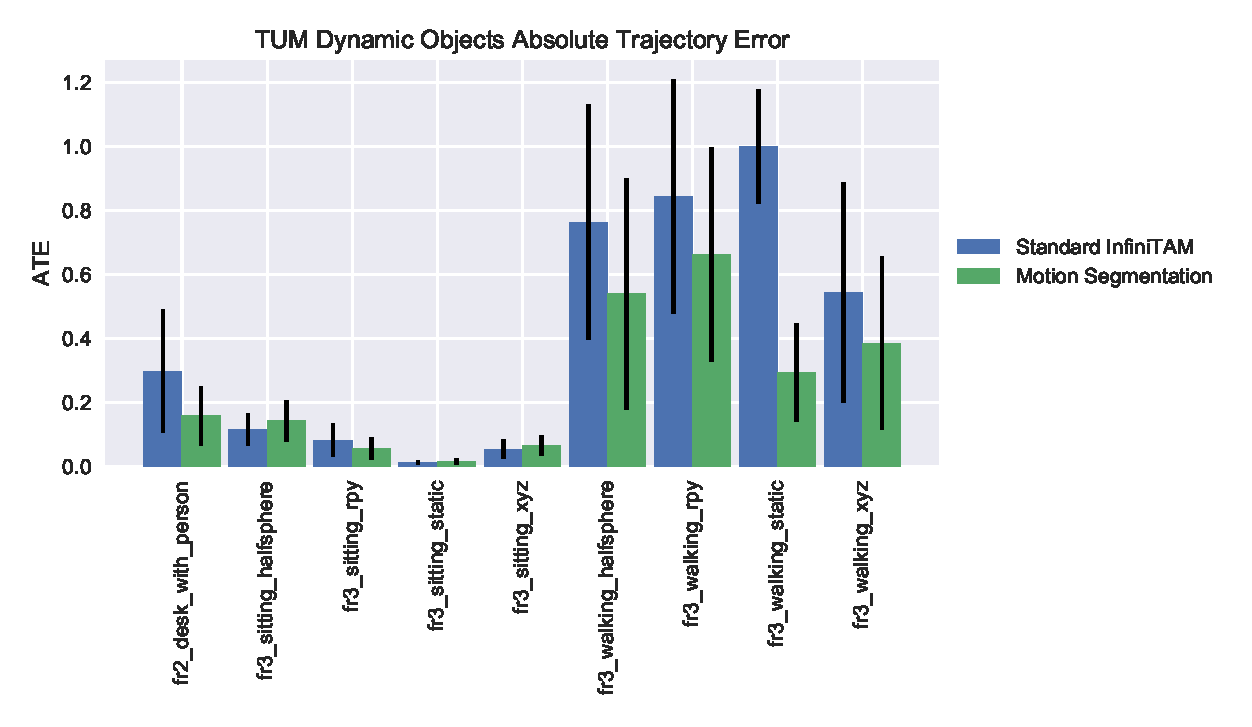
\includegraphics[width=\linewidth]{figures/moseg/ate.eps}
  \caption{Absolute Trajectory Error for the TUM Dynamic Scenes dataset.}
\end{figure}

In addition to evaluating quantitatively in terms of Absolute Trajectory Error,
additional results are provided in terms of Relative Trajectory Error
\cite{Sturm2012}. RTE measures the relative pose error over a fixed time
interval, with the final score being the RMSE over all time windows. RTE results
are provided in Table \ref{tbl:moseg_rte} and visualised in Figure
\ref{fig:moseg_rte}.

\begin{table}[h]
  \label{tbl:moseg_rte}
\begin{center}
  \begin{tabular}{l@{\hskip 1cm} c c}
    \emph{TUM Standard Sequence Name} & \emph{MoSeg} RTE & \emph{Baseline} RTE \\
    \midrule
    \textsf{fr2-desk-with-person} & \textbf{0.023 \std{0.030}} & 0.026 \std{0.037}\\
    \textsf{fr3-sitting-static} & 0.010 \std{0.008} & \textbf{0.010 \std{0.008}}\\
    \textsf{fr3-sitting-xyz} & 0.028 \std{0.017} & \textbf{0.028 \std{0.017}}\\
    \textsf{fr3-sitting-halfsphere} & \textbf{0.031 \std{0.033}} & 0.032 \std{0.029}\\
    \textsf{fr3-sitting-rpy} & 0.073 \std{0.061} & \textbf{0.067 \std{0.065}}\\
    \textsf{fr3-walking-static} & \textbf{0.082 \std{0.140}} & 0.163 \std{0.308}\\
    \textsf{fr3-walking-xyz} & 0.410 \std{0.262} & \textbf{0.300 \std{0.252}}\\
    \textsf{fr3-walking-halfsphere} & \textbf{0.245 \std{0.320}} & 0.305 \std{0.374}\\
    \textsf{fr3-walking-rpy} & 0.482 \std{0.456} & \textbf{0.406 \std{0.364}}\\
  \end{tabular}
\end{center}
\caption{The Relative Trajectory Error (RTE) results (in metres, lower is better
  ) achieved by the proposed approach in comparison to the baseline InfiniTAM
  \cite{Prisacariu2014} framework on a variety of the standard sequences from
  the TUM RGBD dataset \cite{Sturm2012}. Results are in the format mean
  $\pm$ standard deviation. The better result (by mean) on each sequence is
  highlighted in bold.}
\end{table}

\begin{figure}[h]
  \label{fig:moseg_rte}
  \centering
  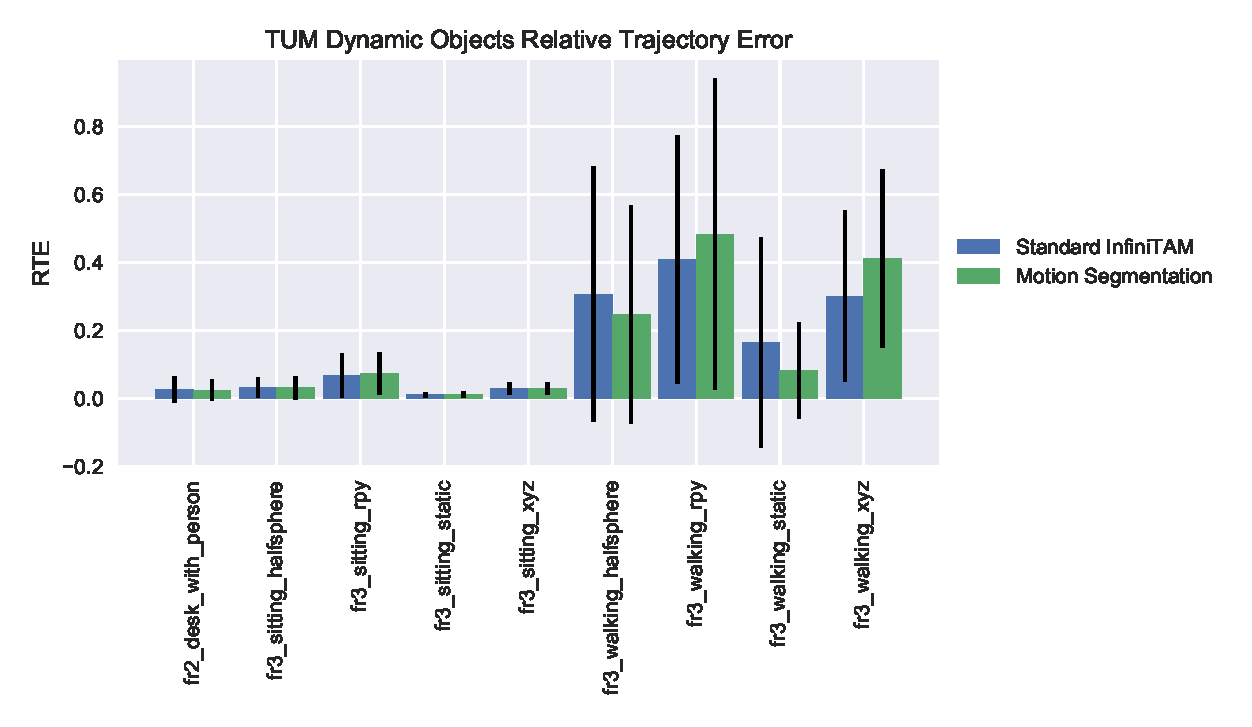
\includegraphics[width=\linewidth]{figures/moseg/rte.eps}
  \caption{Relative Trajectory Error for the TUM Dynamic Scenes dataset.}
\end{figure}

\section{Application to Semantic Scene Understanding}
\label{sec:moseg_semantic}
The dynamic scene handling approach described in \ref{sec:moseg_dynamic_fusion}
can be used to prevent moving objects from being integrated into the static
scene model, but for many applications, e.g. mobile robotics, there is an
additional need to understand what objects are present in the scene and where
they are.

In this section, it is therefore show that classifiers may be trained for the
moving objects and used to recognise new instances of those objects as they
enter the scene.

The Voxel Blocks in the Dynamic Model that were identified as ``unstable''
provide a natural representation of the dynamic parts of the scene. Where
multiple dynamic objects are present, they can be separated by finding the
connected components of these Voxel Blocks. For each object, a one-class Support
Vector Machine (SVM) with a Polynomial Kernel is trained and used to recognise
new instances of the object.

On seeing a new object, the system first tries to classify the object as one
that has already been seen using all of the existing SVMs. If this fails, the
system generates a label for the object and trains a new SVM for it. To make the
training examples for the object, points are uniformly sampled from the object's
surface (Voxels in the object's component that belong to the Zero Level Set) and
compute Fast Point Feature Histogram (FPFH) descriptors \cite{Rusu2009} 
at those points. FPFH descriptors are geometric features that provide a
per-point statistic of the curvature within some neighbourhood of the point
(empirically, a $2.5$cm radius around the point was used).

Figure \ref{fig:moseg_recognition} shows an example of this training and
prediction process for dynamic objects.

\begin{figure}[h]
  \label{fig:moseg_recognition}
  \centering
  \begin{tabular}{ccc}
    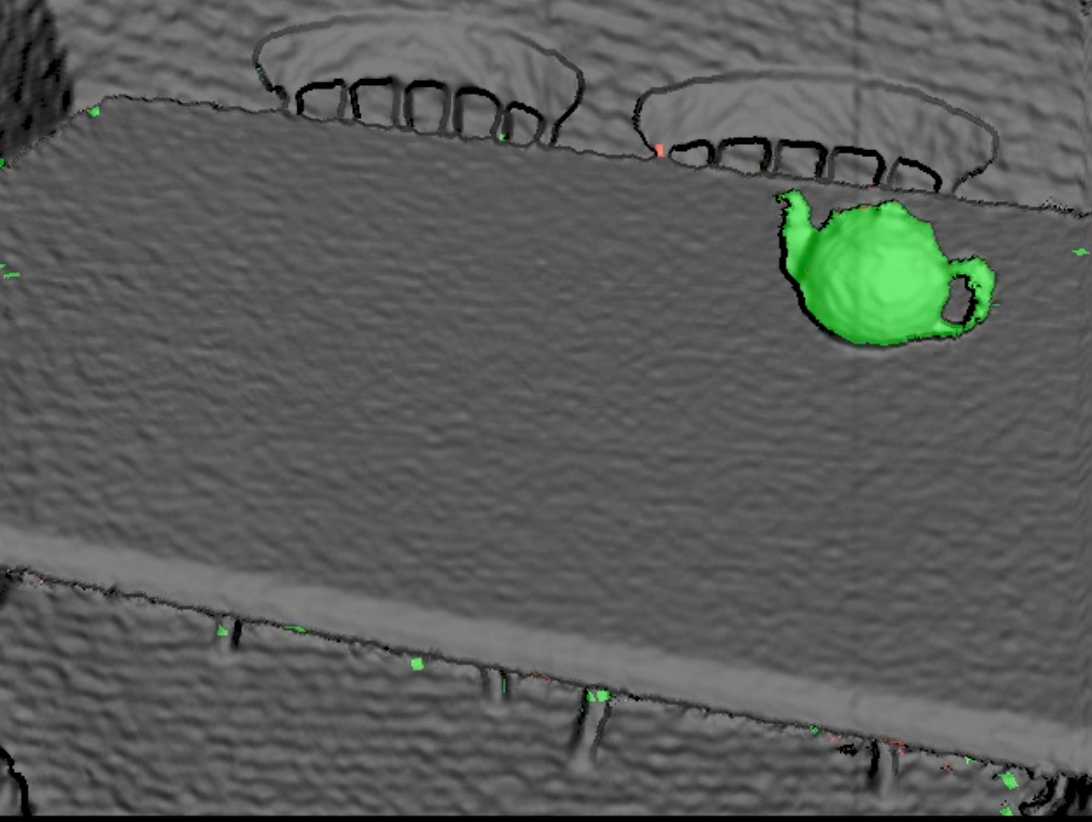
\includegraphics[width=.28\linewidth]{figures/moseg/objects1.png} &
    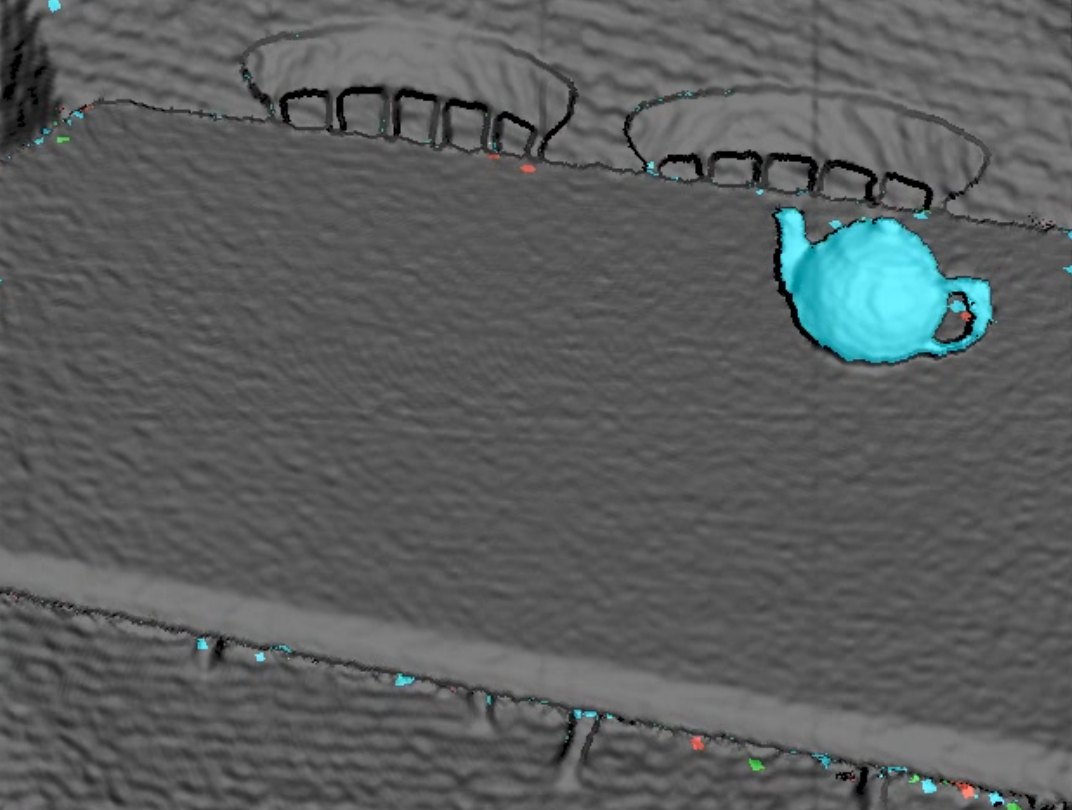
\includegraphics[width=.28\linewidth]{figures/moseg/objects2.png} &
    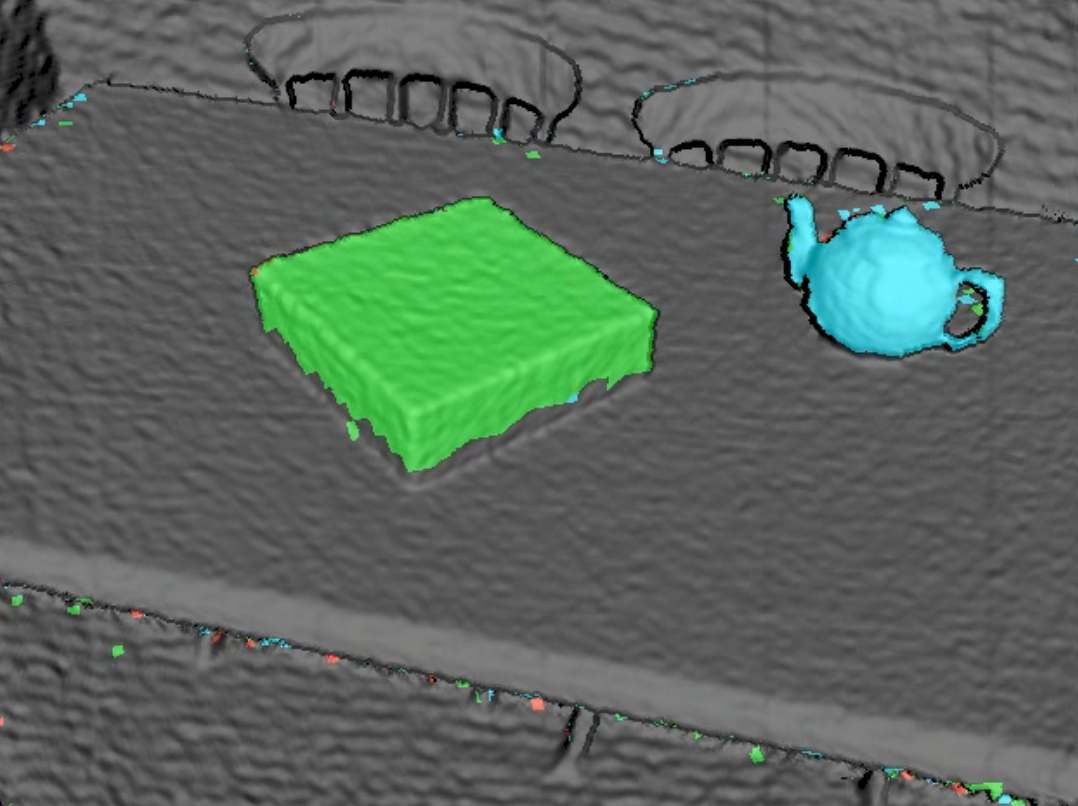
\includegraphics[width=.28\linewidth]{figures/moseg/objects3.png} \\ 
    (a) & (b) & (c) \\
    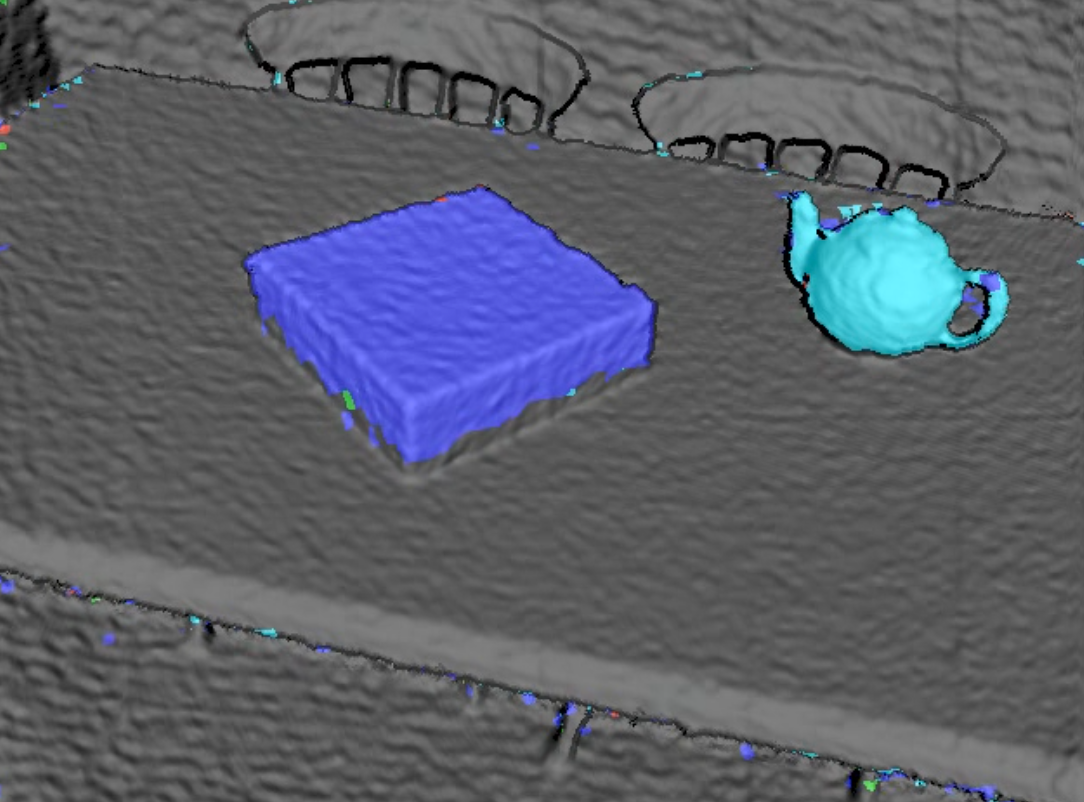
\includegraphics[width=.28\linewidth]{figures/moseg/objects4.png} &
    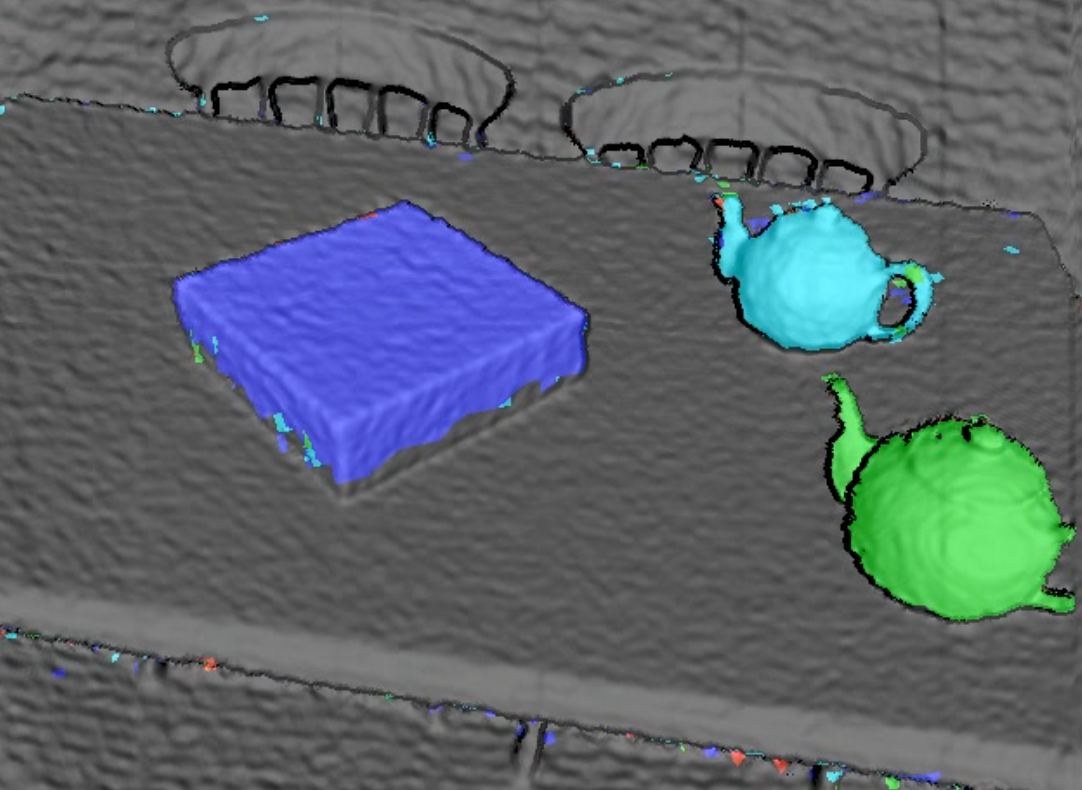
\includegraphics[width=.28\linewidth]{figures/moseg/objects5.png} &
    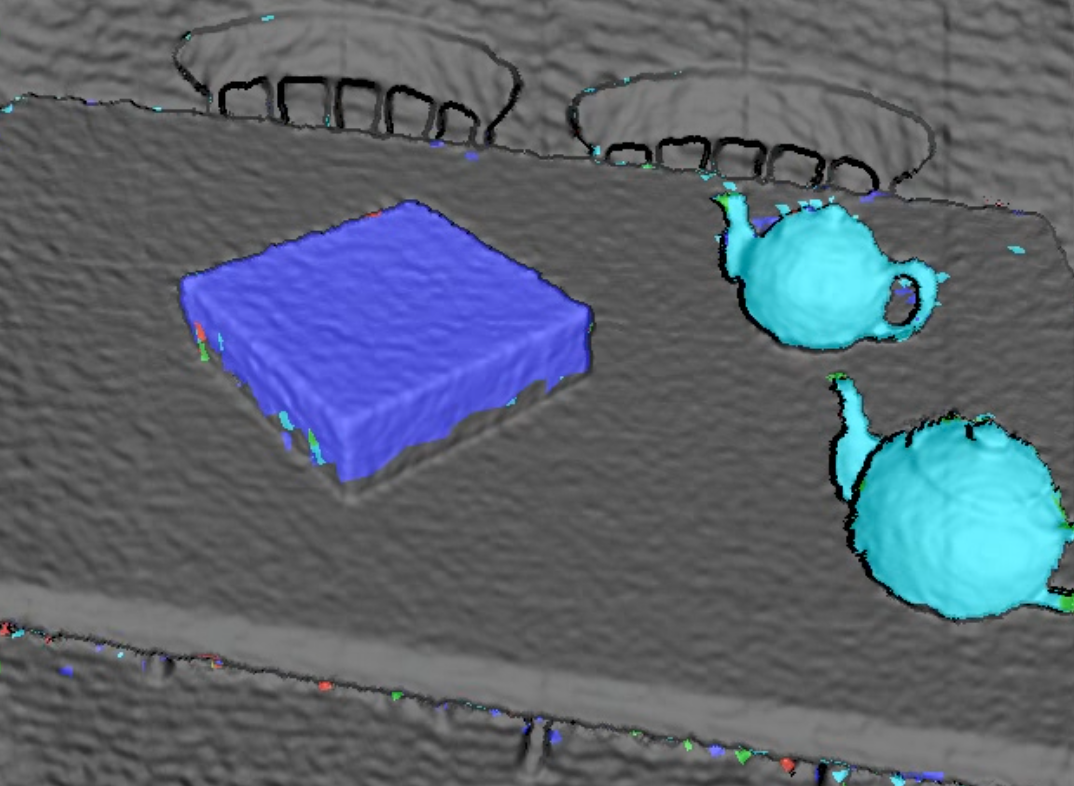
\includegraphics[width=.28\linewidth]{figures/moseg/objects6.png} \\ 
    (d) & (e) & (f) \\
  \end{tabular}
  \caption{An example of the training and prediction process for dynamic
    objects:
    (a) a teapot is placed in the scene;
    (b) the teapot is recognised as a new object and an SVM is trained for it;
    (c) a box is placed in the scene; (d) the box is recognised as being
    distinct from the teapot, and a separate SVM is trained for it;
    (e); another teapot is placed in the scene; (f) the new teapot is recognised
    as being a teapot rather than a box, and is labelled accordingly.}
\end{figure}